\section{Aufbau der Einzelbauteile}

\subsection{OpenSCAD Java Interface}
Für die erleichterte Erstellung von OpenScad Objekten wurde ein Java Interface \icode{ScadObject} erstellt, welches alle für das Projekt wichtigen Befehle enthält.
Die Methode \icode{toString()} stellt in den Klassen des Interfaces die Übergabe des OpenSCAD Befehlsstrings da.
So kann man z.B. mit der Klasse \icode{Cube} einen Quader mit Länge, Höhe und Breite erstellen der dann wie folgt mit \icode{Cube.toString()} in einen String konvertiert wird:\\
\icode{cube([Länge, Breite, Höhe]);}\\
\begin{Bild}{Ergebnis von \icode{new Cube(3, 4, 5).toString()}}
	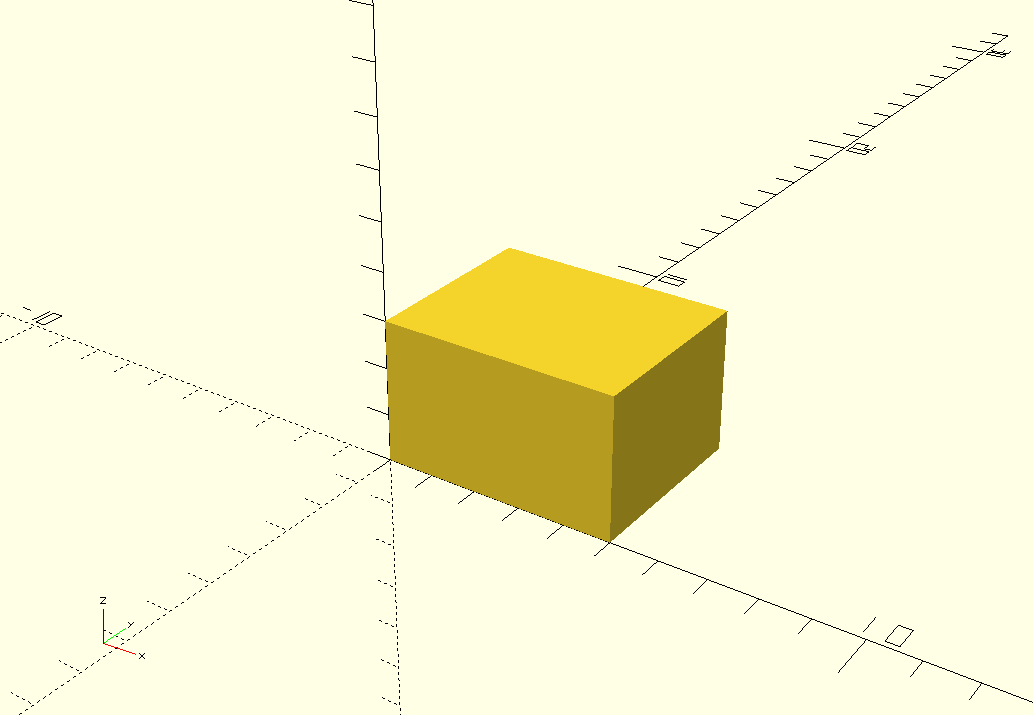
\includegraphics[width = 120mm]{Bilder/Quader}
\end{Bild}



\subsection{Corner}
\subsection{Wall}
\subsection{BasePlate}